\title{ Advanced libMesh Finite Element Spaces}
\maketitle

%%%%%%%%%%%%%%%%%%%%%%%%%%%%%%%%%%%%%%%%%%%%%%%%%%%%%%%%%%%%%%%%%%%%%
\begin{foil}{Lid-Driven Cavity}

The lid-driven cavity provides an adaptivity-friendly divergence-free
shear-thinning 2D Navier-Stokes test: a square domain has zero
velocity enforced on three sides and a constant lateral velocity along
the top.

\begin{center}
%$\vu = (-1, 0)$

%$\vu = 0\;$
\fbox{
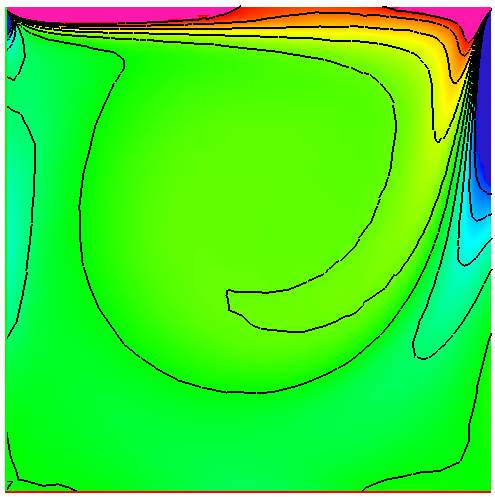
\includegraphics[width=.4\textwidth]{figs/Re500Eta10AdaptiveVorticity}
}
%$\; \vu = 0$
\end{center}

\end{foil}


%%%%%%%%%%%%%%%%%%%%%%%%%%%%%%%%%%%%%%%%%%%%%%%%%%%%%%%%%%%%%%%%%%%%%
\begin{foil}{Corner Singularities}

Because the velocity boundary conditions are discontinuous at the
corners, the streamfunction's first derivative is also discontinuous
and its second derivatives are singular.  As $r \rightarrow 0$,

\vspace{-2em}
\begin{eqnarray*}
\psi(r,\theta) & = & \frac{r}{\pi^2 - 4}
\left( -\pi^2 \sin(\theta) + 2 \pi \theta \sin(\theta) + 
4 \theta \cos(\theta) \right) \\
\vorticity(r, \theta) & = & \frac{1}{(\pi^2 - 4) r}
\left( 4 \pi \cos(\theta) - 8 \sin(\theta) \right)
\end{eqnarray*}
\vspace{-2em}

Without removing these singularities analytically, finite element
simulations at high Reynolds numbers and on coarse meshes are often
corrupted by numerical oscillation.

\end{foil}

%%%%%%%%%%%%%%%%%%%%%%%%%%%%%%%%%%%%%%%%%%%%%%%%%%%%%%%%%%%%%%%%%%%%%
\begin{foil}{Adaptive Cavity Solution}

\begin{center}
$\mbox{Re} = 500$, Extended Williamson fluid, 
$\nu_\infty/\nu_0 = 0.1$

\fbox{
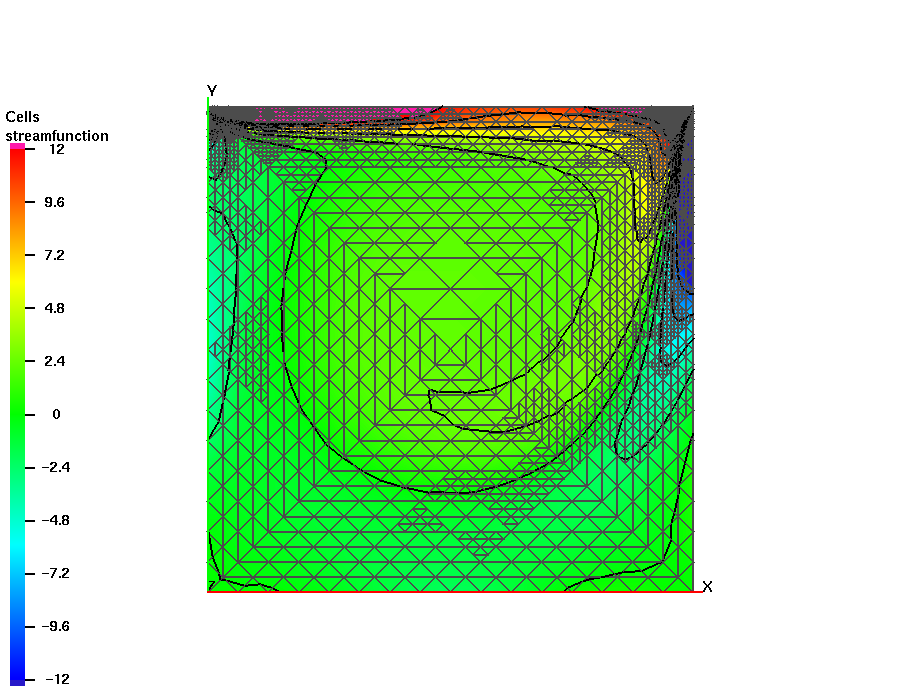
\includegraphics[width=.7\textwidth]{figs/Re500Eta10AdaptiveAll}
}
\end{center}

\end{foil}


%%%%%%%%%%%%%%%%%%%%%%%%%%%%%%%%%%%%%%%%%%%%%%%%%%%%%%%%%%%%%%%%%%%%%
\begin{foil}{Driven Cavity Convergence}

\begin{center}
$\mbox{Re} = 500$, Extended Williamson fluid, 
$\nu_\infty/\nu_0 = 0.1$

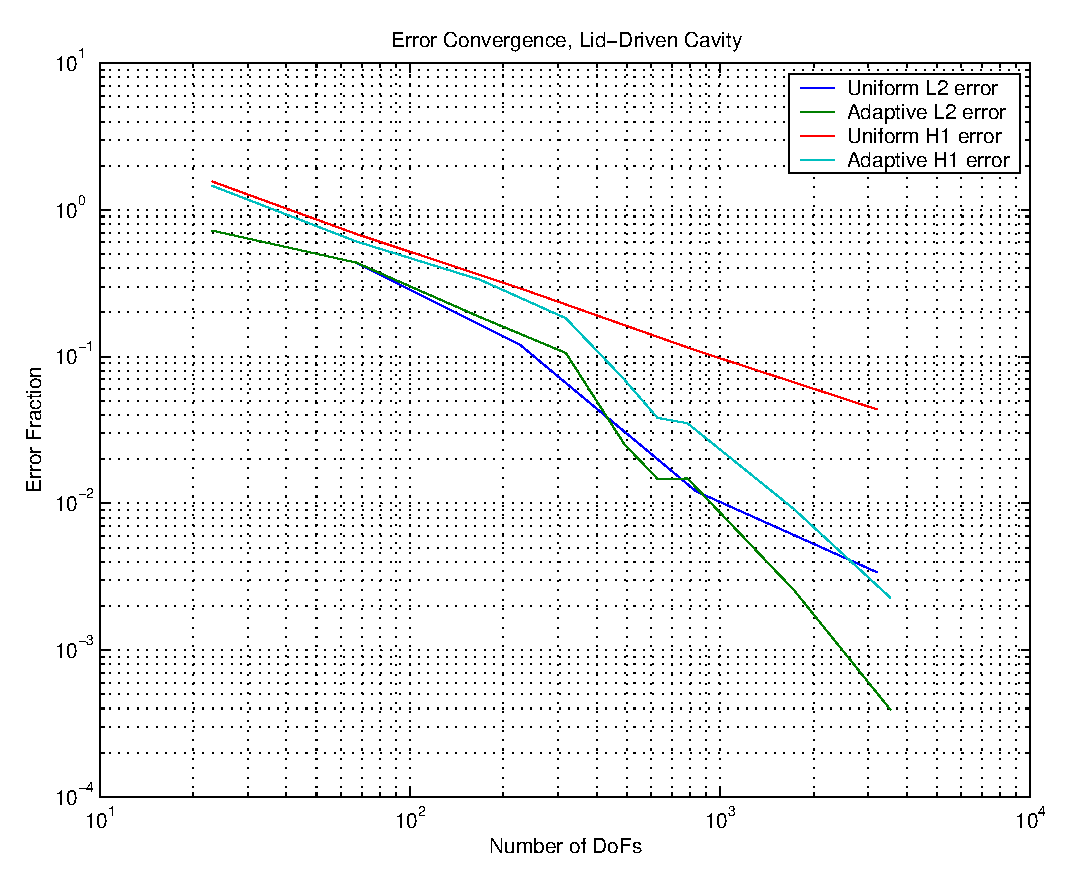
\includegraphics[width=.7\textwidth]{figs/cavityerror}
\end{center}

\end{foil}


%%%%%%%%%%%%%%%%%%%%%%%%%%%%%%%%%%%%%%%%%%%%%%%%%%%%%%%%%%%%%%%%%%%%%
\begin{foil}{Degree of Freedom Handling}

\begin{center}
\fbox{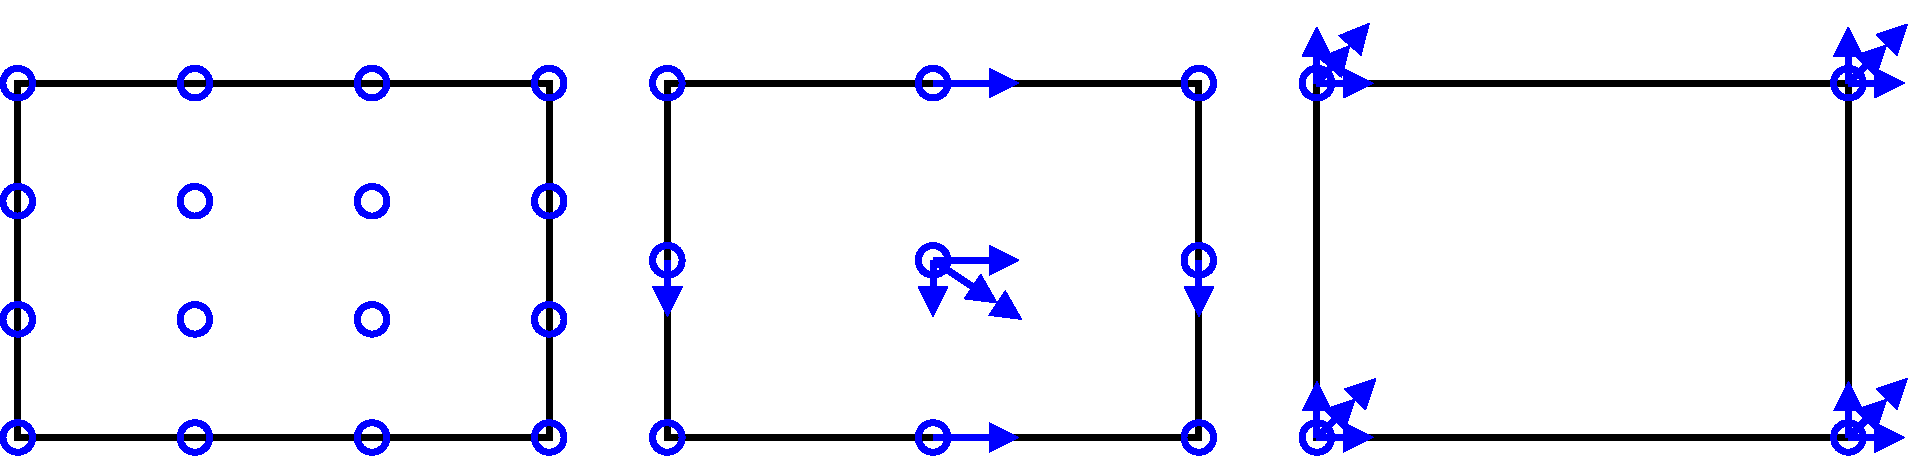
\includegraphics[width=.9\textwidth]{figs/hierarchic}}
\end{center}

\begin{itemize}
  \item Nodes are mapping coordinates
  \item Nodes are topological entities
  \item Nodes are degree-of-freedom objects
\end{itemize}

\end{foil}

%%%%%%%%%%%%%%%%%%%%%%%%%%%%%%%%%%%%%%%%%%%%%%%%%%%%%%%%%%%%%%%%%%%%%
\begin{foil}{Divergence-free Elements}
Replacing $\vec{v}_i$ with $\nabla \times \vec{\phi}_i$ in the
divergence-free flow equations, we find integrated products of second
derivatives of $\vec{\phi}_i$.

The linear Dirichlet problem is well-posed only in an affine space to
$H^2_0(\Omega)$, so any Galerkin finite element approximation must
use $H^2$ conforming functions as well.

A $C^1$ continuous (and $C^n$ bounded, therefore $W^{2,p}$ conforming)
finite element is needed:

\begin{itemize}
	\item Powell-Sabin 6-split triangle
	\item Powell-Sabin-Heindl 12-split triangle
	\item Clough-Tocher 3-split triangle
\end{itemize}
\end{foil}



%%%%%%%%%%%%%%%%%%%%%%%%%%%%%%%%%%%%%%%%%%%%%%%%%%%%%%%%%%%%%%%%%%%%%
\begin{foil}{Macroelements}

Constraining a polynomial triangle to $C^1$ continuity along edges
requires a higher polynomial degree (quintics) than is desired for
many approximations.  Instead, we can construct a macroelement by
subdividing the triangle, using piecewise polynomial functions, and
adding continuity constraints along interior edges.

\begin{center}
\fbox{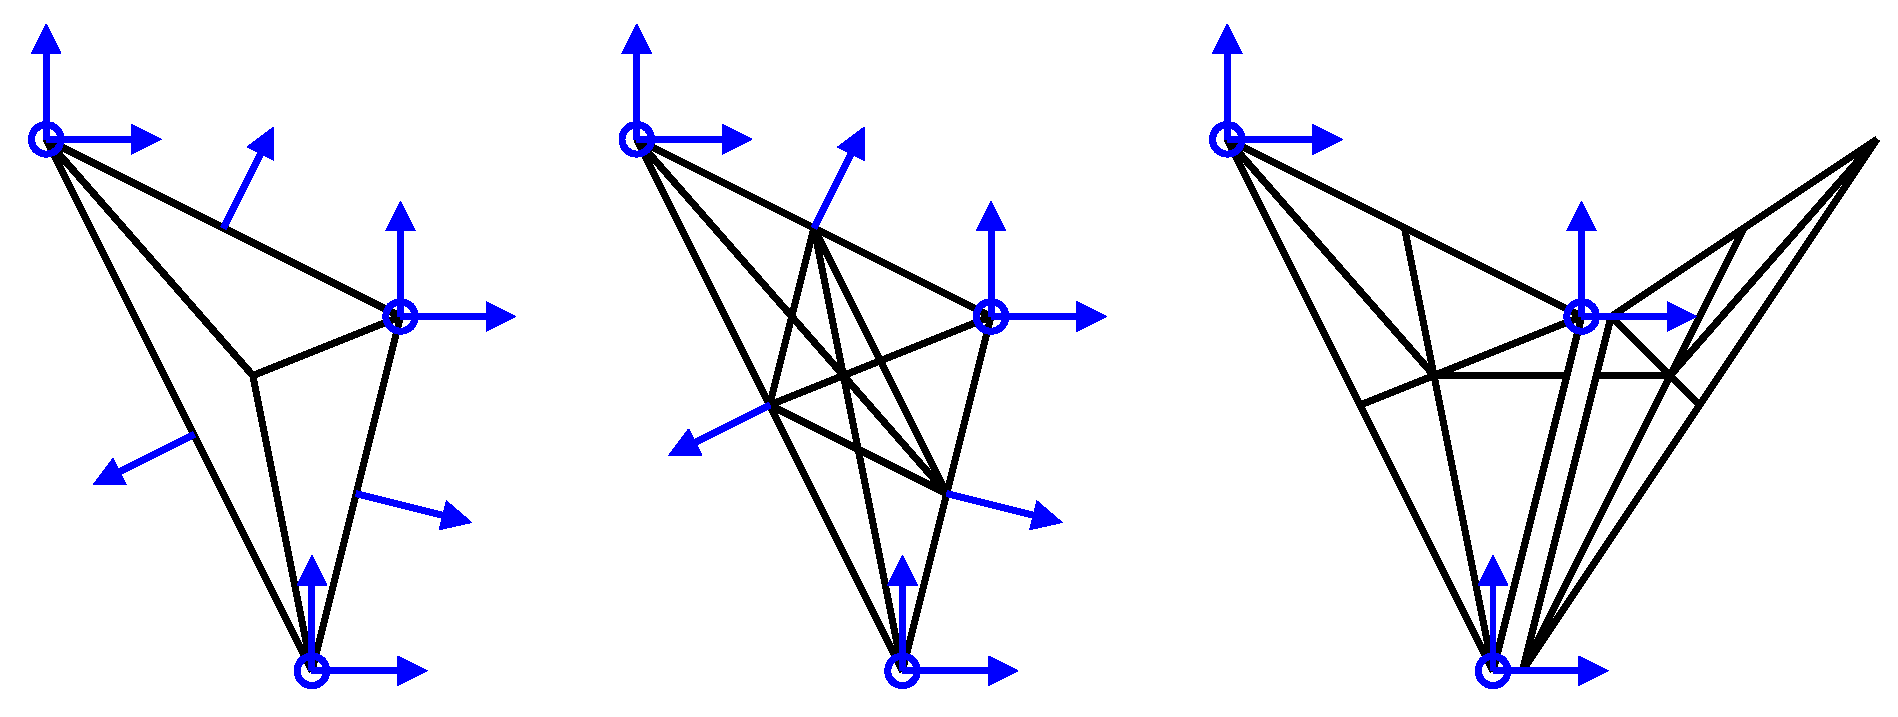
\includegraphics[width=.9\textwidth]{figs/triangles}}
\end{center}

% Mention additional ``raw'' degrees of freedom

% Mention spectral methods

\end{foil}



%%%%%%%%%%%%%%%%%%%%%%%%%%%%%%%%%%%%%%%%%%%%%%%%%%%%%%%%%%%%%%%%%%%%%
\begin{foil}{Powell-Sabin 6-split}
\begin{center}
\fbox{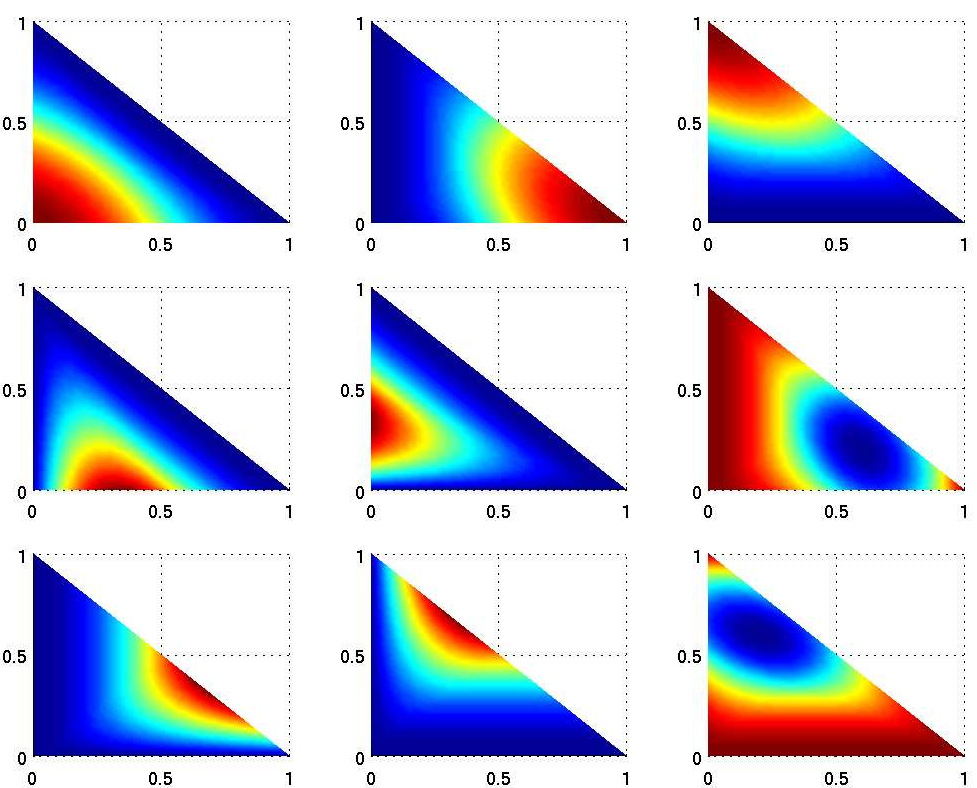
\includegraphics[width=.7\textwidth]{figs/Basis_psrt}}
\end{center}
\end{foil}

\begin{foil}{Powell-Sabin-Heindl 12-split}
\begin{center}
\fbox{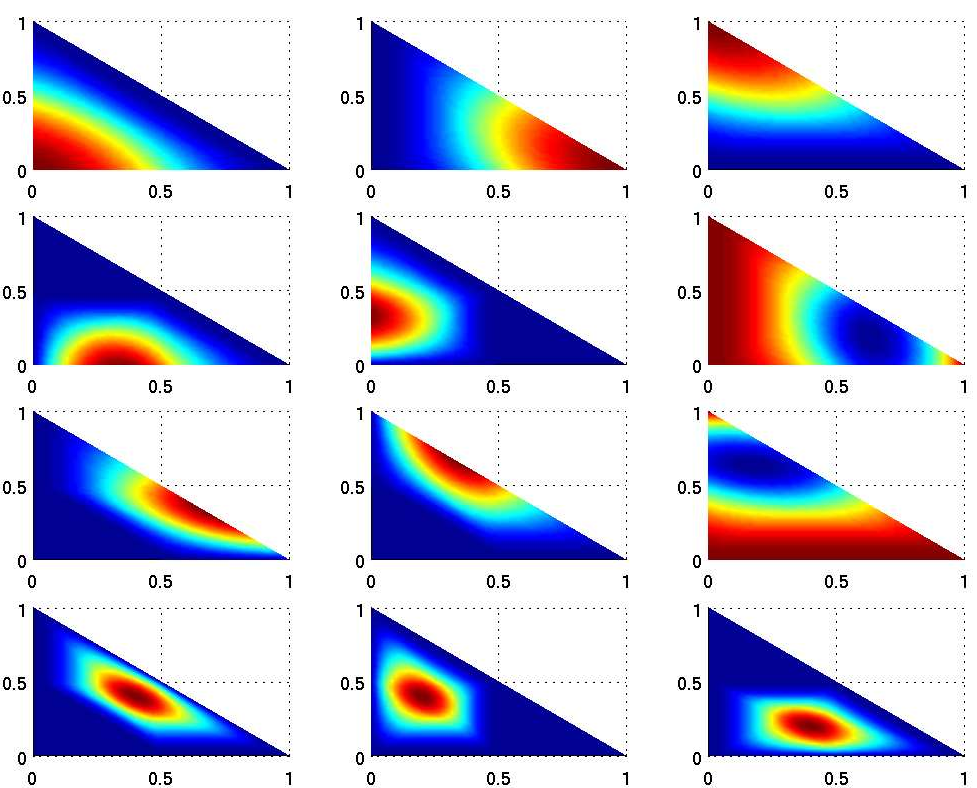
\includegraphics[width=.7\textwidth]{figs/Basis_hrt}}
\end{center}
\end{foil}

\begin{foil}{Clough-Tocher 3-split}
\begin{center}
\fbox{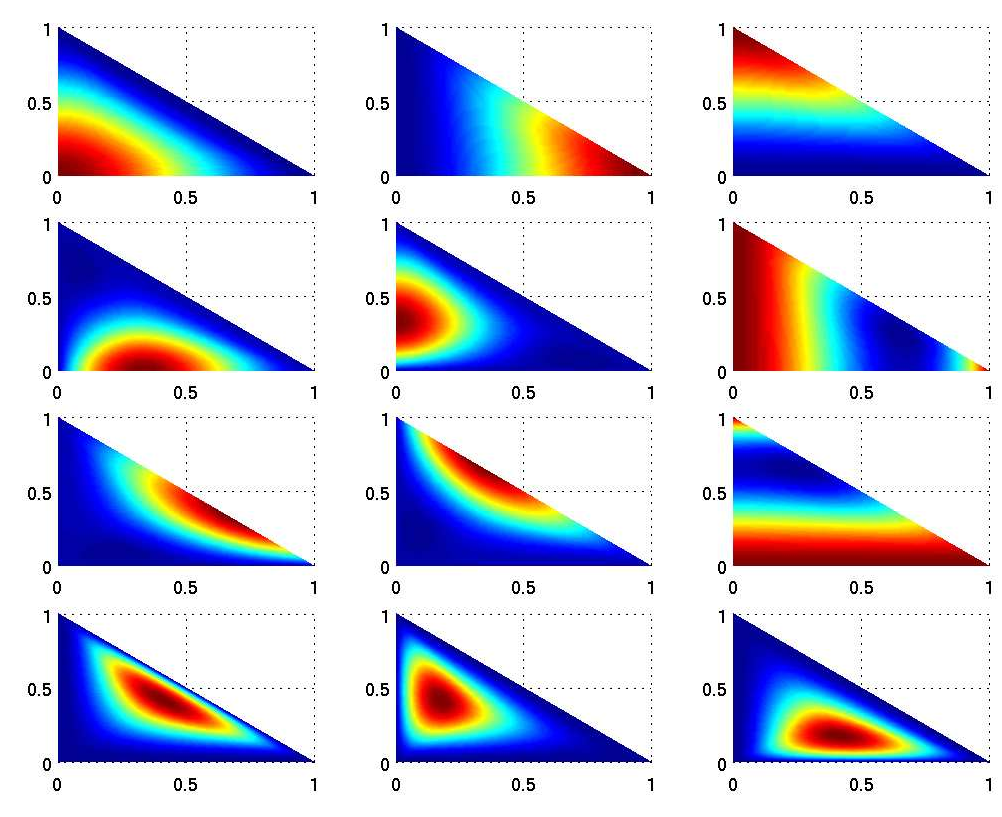
\includegraphics[width=.7\textwidth]{figs/Basis_ctrt}}
\end{center}
\end{foil}

%%%%%%%%%%%%%%%%%%%%%%%%%%%%%%%%%%%%%%%%%%%%%%%%%%%%%%%%%%%%%%%%%%%%%
\begin{foil}{Adaptive Macroelements}

Nonconforming meshes are only stable if solutions are not ``locked''
at hanging nodes.  Function spaces on the sides of fine elements must
be supersets of function spaces on the adjoining sides of coarse
elements.

\begin{center}
\fbox{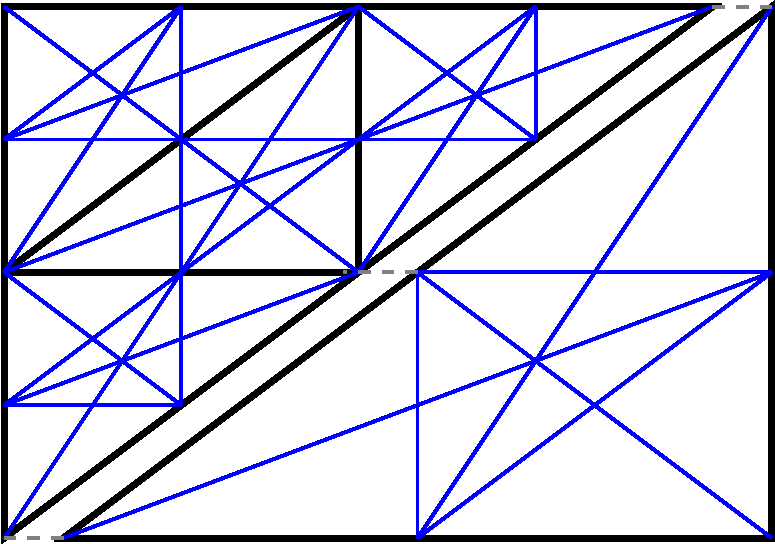
\includegraphics[width=.4\textwidth]{figs/adaptive_psh12}}
\fbox{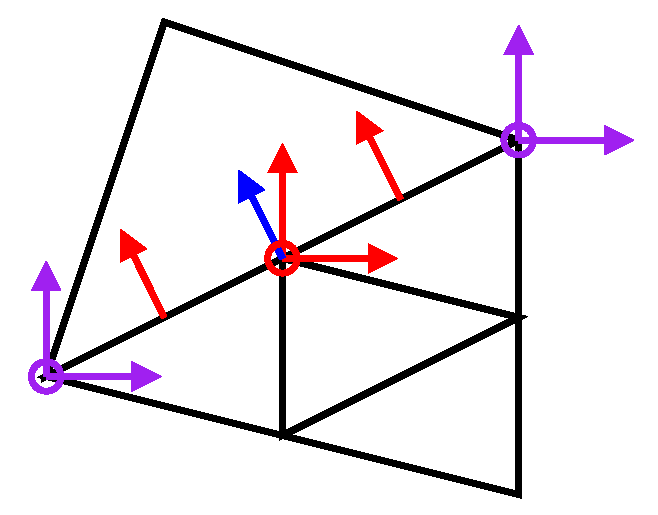
\includegraphics[width=.4\textwidth]{figs/hanging_node}}
\end{center}

\end{foil}


%%%%%%%%%%%%%%%%%%%%%%%%%%%%%%%%%%%%%%%%%%%%%%%%%%%%%%%%%%%%%%%%%%%%%
\begin{foil}{Hanging Node Constraints}

Adaptive mesh refinement creates a non-conforming mesh.  Forming a
$C^1$ conforming function space requires constraining hanging node
degrees of freedom on fine elements in terms of degrees of freedom on
coarse parent elements.

\vspace{-3em}
%\setlength{\parindent}{0pt}
%\zerolistvertdimens
\begin{minipage}[h]{.45\textwidth}
  \begin{figure}[h]
    \begin{center}
      \vspace{-2em}
      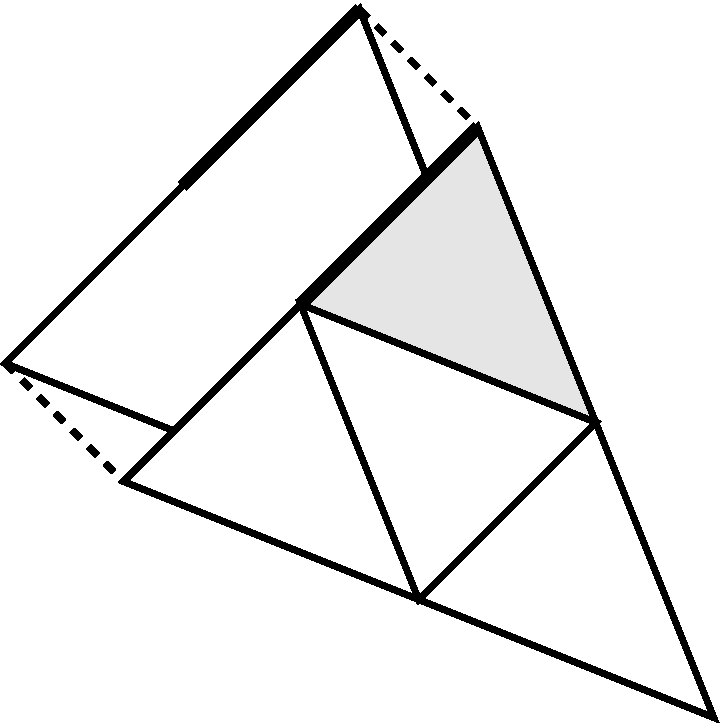
\includegraphics[width=.5\textwidth]{figs/adaptive}
    \end{center}
  \end{figure}
\end{minipage}
\begin{minipage}[h]{.45\textwidth}
\begin{eqnarray*}
u^F & = & u^C \\
\sum_i u_i^F \phi_i^F & = & \sum_j u_j^C \phi_j^C \\
A_{ki} u_i & = & B_{kj} u_j \\
u_i & = & A_{ki}^{-1} B_{kj} u_j \\
\end{eqnarray*}
\end{minipage}
\vspace{-3em}

Element-independent matrices can be formed using an appropriate inner
product:
\vspace{-2em}
\begin{eqnarray*}
A_{ki} & \equiv & (\phi_i^F, \phi_k^F) \\
B_{kj} & \equiv & (\phi_j^C, \phi_k^F) \\
\end{eqnarray*}
\vspace{-4em}

($L_2$ integrated values for $C^0$ continuity, values and fluxes for
$C^1$ continuity)
\end{foil}

%%%%%%%%%%%%%%%%%%%%%%%%%%%%%%%%%%%%%%%%%%%%%%%%%%%%%%%%%%%%%%%%%%%%%
\begin{foil}{Solution Projections}

A good library projection function is:

\begin{itemize}
	\item Locally computable
	\item Uniquely defined
	\item Independent of element type
\end{itemize}

Global Hilbert projections are not locally computable.
Element projections are not uniquely defined.
Pointwise evaluations are not FE independent.

\end{foil}


%%%%%%%%%%%%%%%%%%%%%%%%%%%%%%%%%%%%%%%%%%%%%%%%%%%%%%%%%%%%%%%%%%%%%
\begin{foil}{Solution Projections}

    \begin{center}
      \vspace{-2em}
      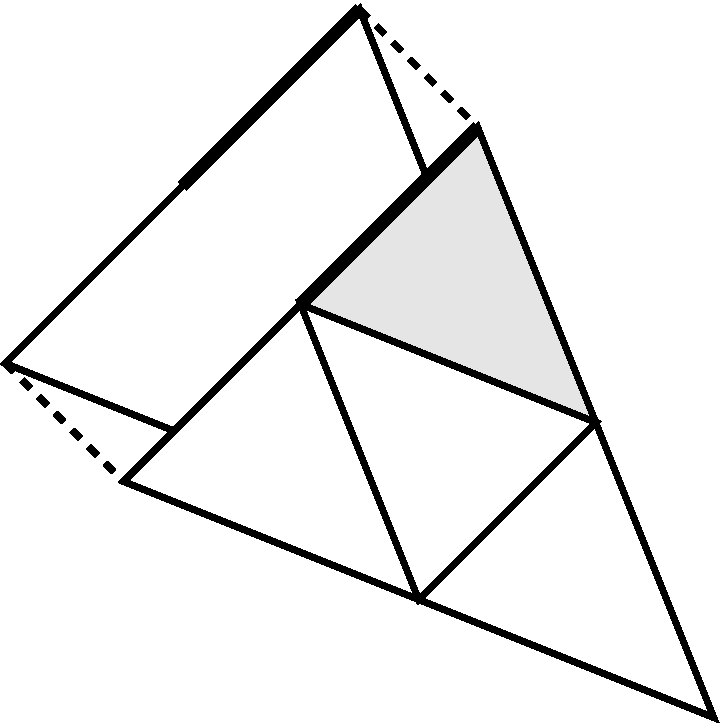
\includegraphics[width=.2\textwidth]{figs/adaptive}
    \end{center}

\begin{itemize}
	\item Copy nodal degrees of freedom
	\item Project edge degrees of freedom
	\item Project face degrees of freedom
	\item Project volume degrees of freedom
\end{itemize}

\end{foil}

%%%%%%%%%%%%%%%%%%%%%%%%%%%%%%%%%%%%%%%%%%%%%%%%%%%%%%%%%%%%%%%%%%%%%
\begin{foil}{Future Development}

\begin{itemize}
	\item Dial-an-operator
	\item Multigrid support
	\item HP adaptivity
	\item Anisotropic adaptivity
\end{itemize}

\end{foil}
